% =====================================================================
% Mục 5. Phân tích phương sai hai chiều (Two-Way ANOVA)
%
% Gói cần có trong file chính: amsmath, amssymb, booktabs, tabularx, array,
%   caption, float, graphicx, listings, xcolor.
% Trước khi \input file này, file chính phải nạp các con số do code sinh ra:
%   % Generated by scripts/reports/report_anova_two_way.py; do not edit by hand.
\newcommand{\AnovaAlpha}{0{,}05}
\newcommand{\AnovaTotalCleaned}{1838}
\newcommand{\AnovaAtiDesktop}{68}
\newcommand{\AnovaAtiLaptop}{0}
\newcommand{\AnovaSampleN}{1770}
\newcommand{\AnovaDfErr}{1766}
\newcommand{\AnovaFCrit}{3{,}847}
\newcommand{\AnovaCellAmdDesktopN}{545}
\newcommand{\AnovaCellAmdLaptopN}{92}
\newcommand{\AnovaCellNvidiaDesktopN}{988}
\newcommand{\AnovaCellNvidiaLaptopN}{145}
\newcommand{\AnovaRawAmdDesktopMean}{141{,}36}
\newcommand{\AnovaRawAmdLaptopMean}{36{,}04}
\newcommand{\AnovaRawNvidiaDesktopMean}{140{,}07}
\newcommand{\AnovaRawNvidiaLaptopMean}{51{,}48}
\newcommand{\AnovaRawAmdDesktopSd}{87{,}55}
\newcommand{\AnovaRawAmdLaptopSd}{28{,}76}
\newcommand{\AnovaRawLeveneW}{75{,}054}
\newcommand{\AnovaRawLeveneP}{$<$ 0{,}001}
\newcommand{\AnovaRawSdRatio}{3{,}04}
\newcommand{\AnovaRawShapiroW}{0{,}9730}
\newcommand{\AnovaRawShapiroP}{$<$ 0{,}001}
\newcommand{\AnovaRawMsErr}{5\,257{,}2}
\newcommand{\AnovaRawFMaker}{1{,}846}
\newcommand{\AnovaRawPMaker}{0{,}1744}
\newcommand{\AnovaRawEtaMaker}{0{,}0010}
\newcommand{\AnovaRawFSeg}{346{,}976}
\newcommand{\AnovaRawPSeg}{$<$ 0{,}001}
\newcommand{\AnovaRawEtaSeg}{0{,}1642}
\newcommand{\AnovaRawFInter}{2{,}580}
\newcommand{\AnovaRawPInter}{0{,}1084}
\newcommand{\AnovaRawEtaInter}{0{,}0015}
\newcommand{\AnovaRawWelchLaptopT}{-3{,}592}
\newcommand{\AnovaRawWelchLaptopP}{$<$ 0{,}001}
\newcommand{\AnovaRawWelchDesktopP}{0{,}7680}
\newcommand{\AnovaLogLeveneW}{15{,}650}
\newcommand{\AnovaLogLeveneP}{$<$ 0{,}001}
\newcommand{\AnovaLogSdRatio}{1{,}30}
\newcommand{\AnovaLogShapiroW}{0{,}9571}
\newcommand{\AnovaLogShapiroP}{$<$ 0{,}001}
\newcommand{\AnovaLogFMaker}{25{,}704}
\newcommand{\AnovaLogPMaker}{$<$ 0{,}001}
\newcommand{\AnovaLogEtaMaker}{0{,}0143}
\newcommand{\AnovaLogFSeg}{625{,}348}
\newcommand{\AnovaLogPSeg}{$<$ 0{,}001}
\newcommand{\AnovaLogEtaSeg}{0{,}2615}
\newcommand{\AnovaLogFInter}{11{,}492}
\newcommand{\AnovaLogPInter}{$<$ 0{,}001}
\newcommand{\AnovaLogEtaInter}{0{,}0065}
\newcommand{\AnovaGeomAmdDesktop}{109{,}9}
\newcommand{\AnovaGeomNvidiaDesktop}{119{,}4}
\newcommand{\AnovaGeomAmdLaptop}{26{,}9}
\newcommand{\AnovaGeomNvidiaLaptop}{40{,}9}
\newcommand{\AnovaLaptopGeomGapPct}{52{,}0}
\newcommand{\AnovaDesktopGeomGapPct}{8{,}7}
\newcommand{\AnovaLogTukeyDeskP}{0{,}1079}
\newcommand{\AnovaLogTukeyLapP}{$<$ 0{,}001}
\newcommand{\AnovaLogWelchDesktopP}{0{,}0348}
\newcommand{\AnovaLogWelchLaptopP}{$<$ 0{,}001}

% (tạo bằng: python scripts/reports/report_anova_two_way.py).
% Không tham chiếu số mục hay số bảng của mục khác; gọi theo nội dung.
% =====================================================================

\section{Phân tích phương sai hai chiều}
\label{sec:anova_two_way}

\subsection{Đặt bài toán và giả thuyết kiểm định}

\textbf{Câu hỏi kiểm định:} \emph{Hãng sản xuất (\texttt{manufacturer}: Nvidia và AMD)
cùng phân khúc thiết bị (\texttt{segment}: Desktop và Laptop) có ảnh hưởng đến công suất
thiết kế tối đa của GPU rời hay không, và chênh lệch giữa hai hãng có phụ thuộc vào phân
khúc (hiệu ứng tương tác) hay không?} Theo mô hình ANOVA hai chiều có lặp ở mức ý
nghĩa $\alpha = \AnovaAlpha$:
\begin{equation}
  Y_{ijk} = \mu + \tau_i + \beta_j + (\tau\beta)_{ij} + \varepsilon_{ijk},
  \qquad \varepsilon_{ijk} \sim \mathcal{N}(0, \sigma^2)\ \text{độc lập},
  \label{eq:two_way_anova}
\end{equation}
{\sloppy với $i \in \{\text{AMD}, \text{Nvidia}\}$ ($a=2$), $j \in \{\text{Desktop},
\text{Laptop}\}$ ($b=2$), $N = \AnovaSampleN$, $df_E = N - ab = \AnovaDfErr$, cùng ràng buộc
$\sum_i \tau_i = \sum_j \beta_j = \sum_i (\tau\beta)_{ij} = \sum_j (\tau\beta)_{ij} = 0$.
Với cỡ mẫu không cân bằng, ta dùng \textbf{Type III SS} và bác bỏ $H_0$ khi $F >
f_{\alpha;\, df_1;\, df_E}$:\par}
\begin{itemize}\setlength{\itemsep}{1pt}\setlength{\parskip}{0pt}
  \item \textbf{Hãng ($SSG$):} $H_{0a}: \tau_1 = \tau_2 = 0$ đối với $H_{1a}: \exists i,\,
    \tau_i \neq 0$; bác bỏ khi $F_a = \mathrm{MSG}/\mathrm{MSE} >
    f_{\AnovaAlpha;\, 1;\, \AnovaDfErr}$.
  \item \textbf{Phân khúc ($SSB$):} $H_{0b}: \beta_1 = \beta_2 = 0$ đối với $H_{1b}:
    \exists j,\, \beta_j \neq 0$; bác bỏ khi $F_b = \mathrm{MSB}/\mathrm{MSE} >
    f_{\AnovaAlpha;\, 1;\, \AnovaDfErr}$.
  \item \textbf{Tương tác A$\times$B ($SSI$):} $H_{0ab}: (\tau\beta)_{ij} = 0\ \forall i,j$
    đối với $H_{1ab}: \exists (i,j),\, (\tau\beta)_{ij} \neq 0$; bác bỏ khi $F_{ab} =
    \mathrm{MSI}/\mathrm{MSE} > f_{\AnovaAlpha;\, 1;\, \AnovaDfErr}$.
\end{itemize}

\subsection{Dữ liệu đầu vào, hiện thực và thống kê mô tả}

{\sloppy Từ tệp đã làm sạch \texttt{gpus\_\allowbreak{}analysis.parquet}
(\AnovaTotalCleaned{} GPU rời đầy đủ biến bắt buộc), hãng ATI có \AnovaAtiDesktop{} mẫu
Desktop nhưng \AnovaAtiLaptop{} mẫu Laptop. Để bảo đảm mọi tổ hợp đều có quan sát, nhóm
lọc về Nvidia và AMD ($n = \AnovaSampleN$, ô nhỏ nhất \AnovaCellAmdLaptopN{} mẫu). Quy
trình được đóng gói trong \texttt{src/\allowbreak{}gpu\_\allowbreak{}power\_\allowbreak{}analysis/\allowbreak{}anova.py}
và gọi chạy tại \texttt{scripts/\allowbreak{}02\_\allowbreak{}anova\_\allowbreak{}two\_\allowbreak{}way.py}
(Đoạn code~\ref{lst:anova_call}).\par}

\begin{lstlisting}[language=Python, label={lst:anova_call},
  caption={Truyền dữ liệu đã làm sạch vào hàm chạy ANOVA hai chiều}]
cleaned = preprocess.load_analysis()
hyp = anova.build_gpu_power_hypotheses(alpha=0.05)
sample, col = anova.prepare_two_way_sample(
    cleaned, "max_power_w", "manufacturer", "segment",
    include_a=("Nvidia", "AMD"), log_transform=False,  # True cho thang log
)
res = anova.run_two_way_anova(
    sample, col, "manufacturer", "segment", ss_type="III"
)
conclusions = anova.conclude_two_way_anova(res, hyp)
\end{lstlisting}

\begin{table}[H]
  \centering
  \caption{Thống kê mô tả công suất GPU trên thang gốc (W) và thang logarit ($\ln$W),
    $n = \AnovaSampleN$}
  \label{tab:anova_cells}
  \scriptsize
  \setlength{\tabcolsep}{3pt}
  \begin{tabular}{@{}lrcrrrr@{}}
    \toprule
    \textbf{Tổ hợp} & \textbf{$n$} & \textbf{Gốc: TB $\pm$ SD}
      & \textbf{Trung vị} & \textbf{Log: TB $\pm$ SD}
      & \textbf{TB nhân (W)} & \textbf{Shapiro $W$ ($p$)$^*$} \\
    \midrule
    \csname @@input\endcsname generated/anova_cells_combined.tex
    \bottomrule
    \multicolumn{7}{@{}p{\linewidth}@{}}{\scriptsize $^*$ Kiểm định Shapiro--Wilk theo
      từng ô trên thang log; trên thang gốc cả bốn ô đều cho $p < 0{,}001$.}
  \end{tabular}
\end{table}

\textbf{Nhận xét Bảng~\ref{tab:anova_cells}.} GPU Desktop của AMD (\AnovaRawAmdDesktopMean{}~W)
và Nvidia (\AnovaRawNvidiaDesktopMean{}~W) cao gấp 2,7--3,7 lần Laptop
(\AnovaRawAmdLaptopMean{}~W và \AnovaRawNvidiaLaptopMean{}~W); hai hãng gần tương đương
trên Desktop, còn trên Laptop Nvidia cao hơn AMD \AnovaRawLaptopGapW{}~W (TB nhân
\AnovaGeomNvidiaLaptop{}~W vs \AnovaGeomAmdLaptop{}~W, chênh \AnovaLaptopGeomGapPct{}\%).

\begin{figure}[H]
  \centering
  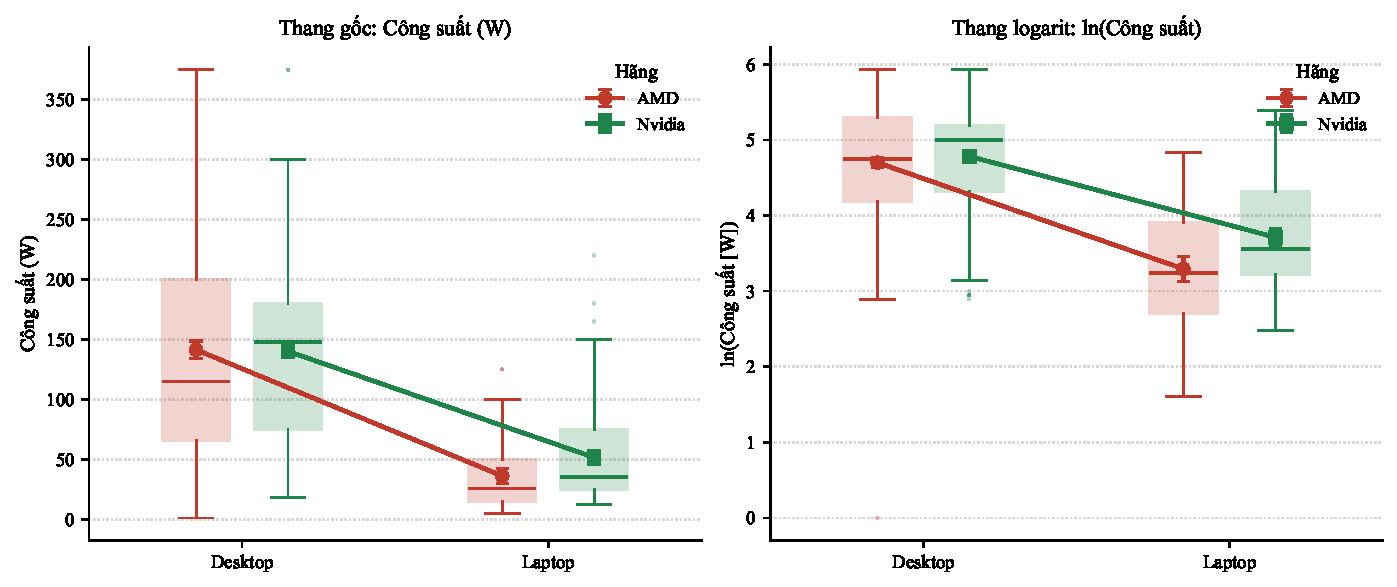
\includegraphics[width=0.80\linewidth]{figures/anova_interaction.pdf}
  \caption{Biểu đồ hộp và đường tương tác trung bình (khoảng tin cậy 95\%) trên thang gốc
    (trái) và thang logarit (phải)}
  \label{fig:anova_interaction}
\end{figure}

\textbf{Nhận xét Hình~\ref{fig:anova_interaction}.} Thang gốc có độ rộng hộp nhóm Desktop
lớn hơn hẳn Laptop và lệch phải mạnh ($\text{SD}_{\max}/\text{SD}_{\min} =
\AnovaRawSdRatio$). Biến đổi logarit làm độ trải bốn nhóm đồng đều hơn rõ rệt và cho thấy
hai đường trung bình không song song (khoảng cách ở Laptop rộng hơn Desktop).

\subsection{Kiểm tra giả định và kết quả ANOVA hai chiều}

{\sloppy \textbf{Kiểm tra ba giả định ANOVA.}\\
\textbf{(1) Tính chuẩn:} trên thang gốc, Shapiro--Wilk bác bỏ ở bốn ô và phần dư
($W = \AnovaRawShapiroW$, $p$~\AnovaRawShapiroP); trên thang log, ô AMD -- Laptop thỏa
chuẩn ($p$~\AnovaLogAmdLapShapiroP), còn phần dư lệch nhẹ do $n$ lớn
($W = \AnovaLogShapiroW$, $p$~\AnovaLogShapiroP) nhưng $n_{ij} \ge
\AnovaCellAmdLaptopN$ bảo đảm kiểm định $F$ bền vững.\\
\textbf{(2) Đồng nhất phương sai:} Levene thang gốc bác bỏ mạnh
($W = \AnovaRawLeveneW$, $p$~\AnovaRawLeveneP, tỉ số SD $= \AnovaRawSdRatio$); thang log
đưa tỉ số SD còn \textbf{\AnovaLogSdRatio{}} ($< 2{,}0$) và giảm $W$ xuống
$\AnovaLogLeveneW$ ($p$~\AnovaLogLeveneP).\\
\textbf{(3) Tính độc lập:} các bản ghi ứng với mẫu GPU độc lập, song một số card dùng
chung kiến trúc nên kết quả được kiểm chứng thêm bằng Welch $t$-test.\par}

\begin{table}[H]
  \centering
  \caption{Kết quả ANOVA hai chiều (Type III SS) trên thang gốc và thang logarit
    ($\alpha = \AnovaAlpha$, $f_{\AnovaAlpha;\, 1;\, \AnovaDfErr} = \AnovaFCrit$)}
  \label{tab:anova_table}
  \footnotesize
  \setlength{\tabcolsep}{4pt}
  \begin{tabular}{@{}lrrrrrr@{}}
    \toprule
    \textbf{Nguồn biến thiên} & \textbf{$SS$} & \textbf{$df$} & \textbf{$MS$}
      & \textbf{$F$} & \textbf{$p$-value} & \textbf{$\eta_p^2$} \\
    \midrule
    \csname @@input\endcsname generated/anova_table_combined.tex
    \bottomrule
    \multicolumn{7}{@{}p{\linewidth}@{}}{\scriptsize $^*$ Với Type III SS cho cỡ mẫu không
      cân bằng, tổng $SSG + SSB + SSI + SSE$ nói chung khác $SST$.}
  \end{tabular}
\end{table}

\textbf{Nhận xét Bảng~\ref{tab:anova_table}.} Trên \textbf{thang gốc} (Panel A), chỉ
phân khúc có ý nghĩa ($F_b = \AnovaRawFSeg > \AnovaFCrit$, $p$~\AnovaRawPSeg, $\eta_p^2 =
\AnovaRawEtaSeg$, bác bỏ $H_{0b}$); hãng ($F_a = \AnovaRawFMaker$, $p$~\AnovaRawPMaker) và
tương tác ($F_{ab} = \AnovaRawFInter$, $p$~\AnovaRawPInter) chưa bác bỏ được
$H_{0a}, H_{0ab}$ do $\mathrm{MSE} = \AnovaRawMsErr$ lớn ở Desktop. Trên \textbf{thang
logarit} (Panel B, $\mathrm{MSE} = \AnovaLogMsErr$), cả ba kiểm định đều vượt $\AnovaFCrit$
(bác bỏ $H_{0a}, H_{0b}, H_{0ab}$): phân khúc mạnh nhất ($F_b = \AnovaLogFSeg$,
\AnovaLogEtaSegPct{}\%, $p$~\AnovaLogPSeg), cùng hãng ($F_a = \AnovaLogFMaker$,
$p$~\AnovaLogPMaker) và \textbf{tương tác} ($F_{ab} = \AnovaLogFInter$,
$p$~\AnovaLogPInter).

\subsection{Hậu kiểm, kiểm chứng hiệu ứng đơn và kết luận}

{\sloppy \textbf{Hậu kiểm Fisher's LSD.} Trên thang logarit ($\mathrm{MSE} =
\AnovaLogMsErr$, $t_{\alpha/2;\, \AnovaDfErr} = \AnovaTCrit$), công thức $\mathrm{LSD}_{ij} =
t_{\alpha/2,\, df_E}\sqrt{\mathrm{MSE}(1/n_i + 1/n_j)}$ phát hiện
\AnovaLogLsdSigCount/6 cặp khác biệt (Laptop: $|\Delta| = \AnovaLogLsdLapDiff >
\AnovaLogLsdLapCrit$; Desktop: $|\Delta| = \AnovaLogLsdDeskDiff > \AnovaLogLsdDeskCrit$),
còn thang gốc ghi nhận \AnovaRawLsdSigCount/6 cặp. Do LSD giữ sai số theo cặp thay vì toàn
họ, Hình~\ref{fig:anova_tukey_ci} kiểm chứng thêm bằng \textbf{Tukey HSD}.\par}

\begin{figure}[H]
  \centering
  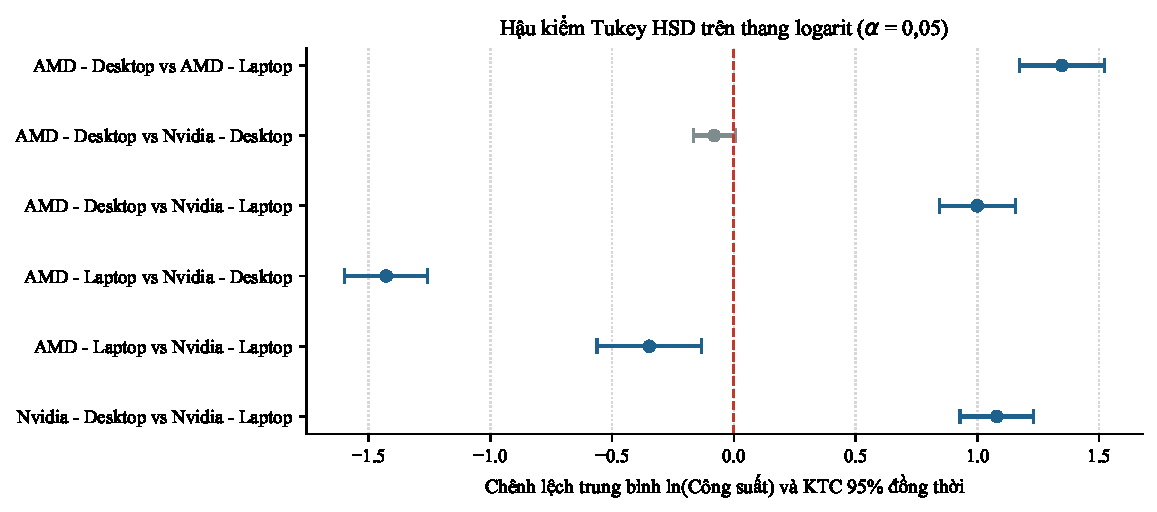
\includegraphics[width=0.62\linewidth]{figures/anova_tukey_ci.pdf}
  \caption{Khoảng tin cậy 95\% đồng thời của hậu kiểm Tukey HSD trên thang logarit}
  \label{fig:anova_tukey_ci}
\end{figure}

\textbf{Nhận xét Hình~\ref{fig:anova_tukey_ci}.} Theo Tukey HSD, 5/6 cặp có khoảng tin
cậy 95\% đồng thời không chứa 0 ($p < 0{,}001$); cặp AMD -- Desktop vs Nvidia -- Desktop
cắt qua 0 ($p$~\AnovaLogTukeyDeskP), còn trên Laptop Nvidia vượt AMD rõ rệt
($p$~\AnovaLogTukeyLapP), khẳng định tương tác.

\begin{table}[H]
  \centering
  \caption{Kiểm định hiệu ứng đơn bằng Welch $t$-test (không cần phương sai bằng nhau)}
  \label{tab:anova_simple_effects}
  \footnotesize
  \setlength{\tabcolsep}{3.5pt}
  \begin{tabular}{@{}llrrrrrr@{}}
    \toprule
    & & \multicolumn{3}{c}{\textbf{Thang gốc (W)}}
      & \multicolumn{3}{c}{\textbf{Thang logarit ($\ln$W)}} \\
    \cmidrule(lr){3-5} \cmidrule(lr){6-8}
    \textbf{Điều kiện} & \textbf{Cặp so sánh} & \textbf{Chênh lệch} & \textbf{$t$}
      & \textbf{$p$-value} & \textbf{Chênh lệch} & \textbf{$t$} & \textbf{$p$-value} \\
    \midrule
    \csname @@input\endcsname generated/anova_simple_effects.tex
    \bottomrule
  \end{tabular}
\end{table}

\textbf{Nhận xét Bảng~\ref{tab:anova_simple_effects}.} Welch $t$-test nhất quán trên hai
thang đo: Desktop cao hơn Laptop rất mạnh ở cả hai hãng ($p < 0{,}001$); trong Laptop,
Nvidia vượt AMD rõ rệt ($t = \AnovaRawWelchLaptopT$, $p$~\AnovaRawWelchLaptopP; thang log
$p$~\AnovaLogWelchLaptopP); trong Desktop, hai hãng tương đương ở thang gốc
($p$~\AnovaRawWelchDesktopP) và lệch nhẹ trên thang log ($p$~\AnovaLogWelchDesktopP,
Tukey HSD không có ý nghĩa).

\textbf{Kết luận trả lời câu hỏi kiểm định ($\alpha = \AnovaAlpha$).} \textbf{Có} ---
trên thang logarit (đã ổn định phương sai), bác bỏ cả $H_{0a}, H_{0b}, H_{0ab}$:
\textbf{hãng} ($p$~\AnovaLogPMaker), \textbf{phân khúc} ($p$~\AnovaLogPSeg) và
\textbf{tương tác} ($p$~\AnovaLogPInter) đều ảnh hưởng có ý nghĩa đến công suất GPU rời
(thang gốc chỉ bác bỏ $H_{0b}$ do phương sai Desktop lớn).\\
\textbf{(1) Nhân tố chủ đạo:} phân khúc chi phối mạnh nhất
(\AnovaRawEtaSegPct{}\%--\AnovaLogEtaSegPct{}\% phương sai cục bộ).\\
\textbf{(2) Tương tác theo tỉ lệ:} trên Desktop hai hãng tương đương
(\AnovaGeomNvidiaDesktop{}~W vs \AnovaGeomAmdDesktop{}~W), còn trên Laptop Nvidia vượt
AMD \AnovaLaptopGeomGapPct{}\% (\AnovaGeomNvidiaLaptop{}~W vs
\AnovaGeomAmdLaptop{}~W).\\
\textbf{(3) Hạn chế:} biến thiên Desktop còn lớn nên cần thêm biến phần cứng khi hồi
quy; dù có chung kiến trúc (\texttt{architecture}), kết luận vẫn vững qua Welch
$t$-test.
